\documentclass[11pt]{article}

\usepackage{graphicx}
\usepackage[top=1in, bottom=1in, left=1in, right=1in]{geometry}

\parindent 0ex

\begin{document}

\twocolumn

\setlength{\columnsep}{25pt}

\title{Valuing Teams by Discounting Future Championships}
\author{Gordon Kamer}
\date{\today}
\maketitle

\section{Introduction}

The stated goal of most general managers and the explicit wish of most fans is for a team to win the World Series and to win it as many times as possible, preferably sooner rather than later. Mathematically, we can put a single number on every team in baseball representing the discounted value of future championships. It is the general manager's job every day to maximize this value. The most valuable team in this metric can be said to be the team best positioned for both today and the future.\\\\
This paper seeks to provide some method for determining a version of this number that is context neutral (not dependent on the division of the team or things like the team's stadium and management).

\section{Team Value}

We can represent team value by the letter $V$. Let $I_i$ be the indicator variable of the event $C_i$ that the team wins the World Series after $i$ years. Let $r$ be the discount rate for championships, $0 < r < 1$. We define $V$ as follows.

\begin{eqnarray*}
V &=& E\left(\sum_{k=0}^{\infty}\frac{I_k}{(1 + r)^k}\right)\\
V &=& \sum_{k=0}^{\infty}\frac{E(I_k)}{(1 + r)^k}\\
V &=& \sum_{k=0}^{\infty}\frac{P(C_k)}{(1 + r)^k}
\end{eqnarray*}

Thus we can solve for championship value if we have some predetermined value $r$, representing the discount rate that we apply, and the championship probability for the team in every year in the future.

\section{Championship Probability}
Predicting the world series winner with $100\%$ certainty just one year in advance is impossible without universally complete information. Predicting it with any kind of certainty years in the future is even more difficult. However, using some assumptions and past data, we can produce some estimate of each team's championship probability.

\subsection{Players and Wins}

Wins Above Replacement (WAR) is the best stat we have to determine the context-neutral contribution of every player on a team. If we sum up the WAR of every player on a team, we get some kind of expected win total of a team. Here we can make our first core assumptions.

\begin{enumerate}
	\item Championship win probability is completely determined by the sum of the individual contributions of the players.
	\item Players' skill does not change predictably between the regular season and the postseason.
\end{enumerate}

I avoid explicitly using WAR because WAR is merely the statistic \textit{du jour} in order to calculate these things, and there are even many different kinds of WAR (like fWAR, bWAR, etc.). We will continually improve that statistic, and no improvement would fundamentally change the meaning of the championship value calculated in this paper.\\\\
The first assumption states that $2 + 2 = 4$. It means that everything we could ever want to know about the team's chances can be determined by looking at the our predictions for the performances of individual players. It also packs some deeper assumptions within it. We will not be making our prediction for championship probability dependent on predictions about other teams\textemdash say, other teams in the same division. We will only look at the players on that specific team.\\\\
The second assumption means that teams that are players in the regular season are expected to be good in the postseason. It also means that we will not take a team's make-up (say, being pitching heavy or having players who have historically performed well in the postseason) as being any more predictive as regular season skill. It is possible to imagine that this assumption could be relaxed, but it would be difficult considering certain assumptions made elsewhere.\\\\
Let $W_j$ be the contribution of the j'th player under team control and let $n_i$ be the number of players under team control during a season $i$ years in the future. $S_i$ is thus the sum of player contributions:
$$S_i = \sum_{j=1}^{n_i}{W_j}$$

And everything we could ever want to know about $P(C_i)$, the championship probability of a team, is given by $S_i$. Practically, we can treat $S_i$ as the sum of individual player WAR values.

\subsection{From Wins to Championships}

We need now to get from the sum of individual player contributions to a championship probability. Let $P(C_i | S_i = s)$ be the probability of winning the championship conditional on the skill of the team (the sum of player contributions). This conditional probability is easier to calculate. Let $f(s)$ be the probability density function of $S_i$, the sum of individual player contributions. We can find the desired marginal probability as follows.
$$P(C_i) = \int_{-\infty}^{\infty}f(s) P(C_i|S_i=s)ds$$
Therefore, in order to calculate $P(C_i)$ for each year, which can give us our team's total championship value, we can use the probability that a team wins given some player contribution sum (practically, the sum of player WAR) in addition to the distribution of $S_i$ for every year in the future.

\section{Championship Win Probability Given Win Sums}

This section attempts to provide some practical estimate to $P(C_i | S_i = s)$, which should not change much from year to year or from team to team. One major challenge is that the playoff format has changed over the years by a large amount, which limits the amount of data we can use. While we'd like to simply fit some logistic function of WAR, we will need to break down the problem into parts and use data from 2000 onward to get a reasonable estimate.\\\\
Let $D_i$ be the event that the team wins the division. Let $W_i$ be the event that the team wins the wild card. Let $R_{i_{j}}$ be the event that the team wins the $j$'th playoff round, given that they've reached that round, where $j$ is $0$ for the wild card game, $1$ for the division series, and so on.
$$P(C_i|S_i) = (P(D_i)+ P(W_i)P(R_{i_0}))\prod_{j=1}^{3}{P(R_{i_{j}})}$$

\subsection{Team Record}

Of course, figuring out precise playoff odds depends on knowing things about other teams, like those in the division. In that case, a simulation might be the best option. For simplicity and to maintain context neutrality, we will ignore that fact when trying to estimate our conditional probability, using only information about the given team.\\\\
Figure 1 displays a linear regression plot of combined batting and pitching WAR vs. win-loss percentage. The data are extremely well modeled by a linear function, as is expected from the construction of the WAR statistic. Moreover, the y-intercept of the regression line is .304, which is quite close to the replacement level team winning percentage of .294 used by BaseballReference; the x-coefficient is .00588, which is close to $\frac{1}{162}$.\\

\begin{figure}
  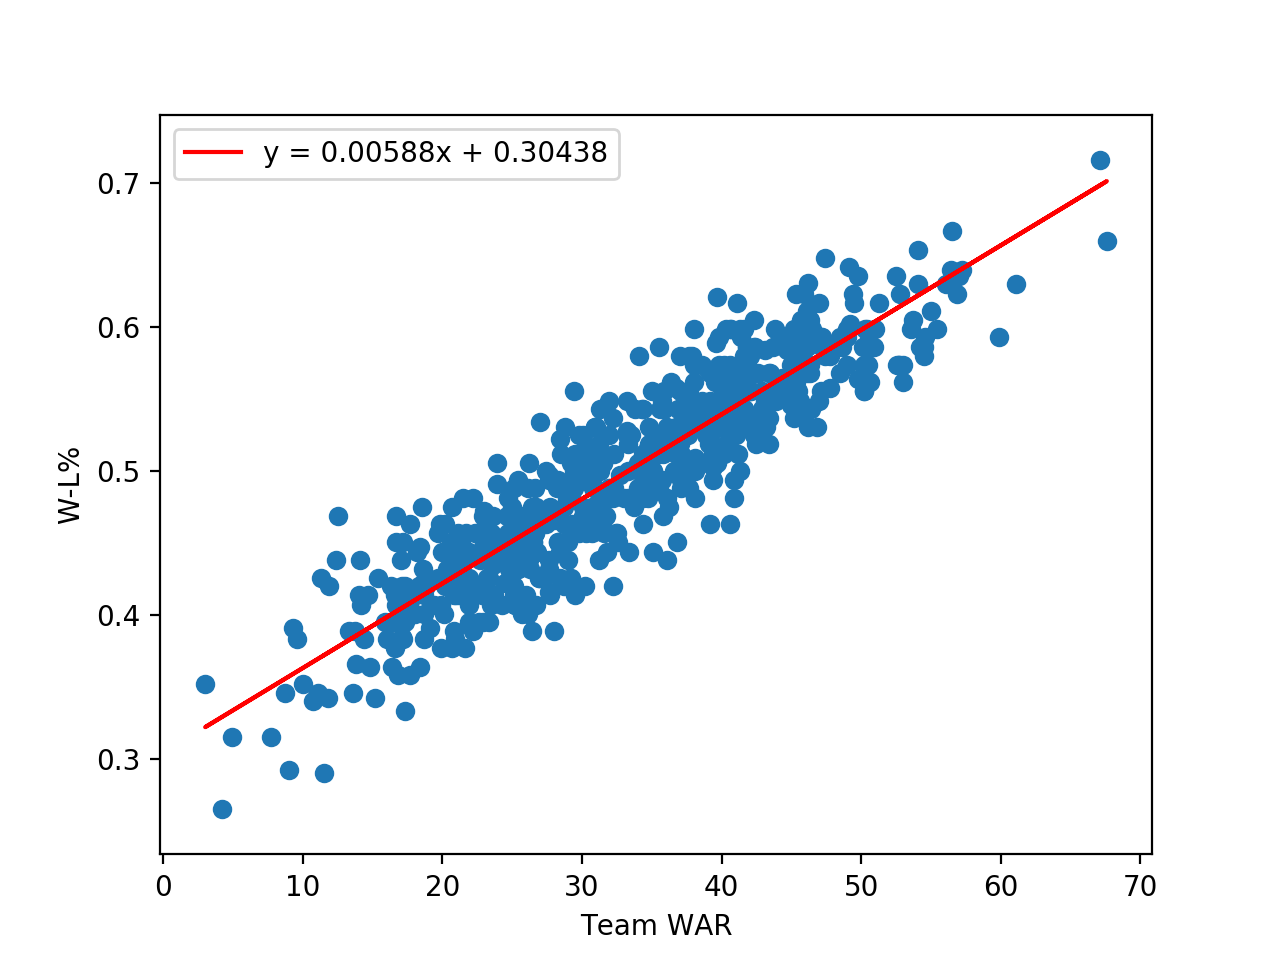
\includegraphics[width=\linewidth]{figure1.png}
  \caption{Predicting team W-L\% from WAR}
  \label{fig:figure1}
\end{figure} 

The important information from this plot is the shape of the residuals, which tells us roughly how accurate WAR is and which gives us a probability distribution for the team's win-loss percentage from the team's WAR. Figure 2 shows a normal distribution with the mean and variance of the residuals from the plot above. The plot also includes dots that represent each residual. The y-coordinates of those dots have had noise added to them so that the density of the dots is easier to see.\\

\begin{figure}
  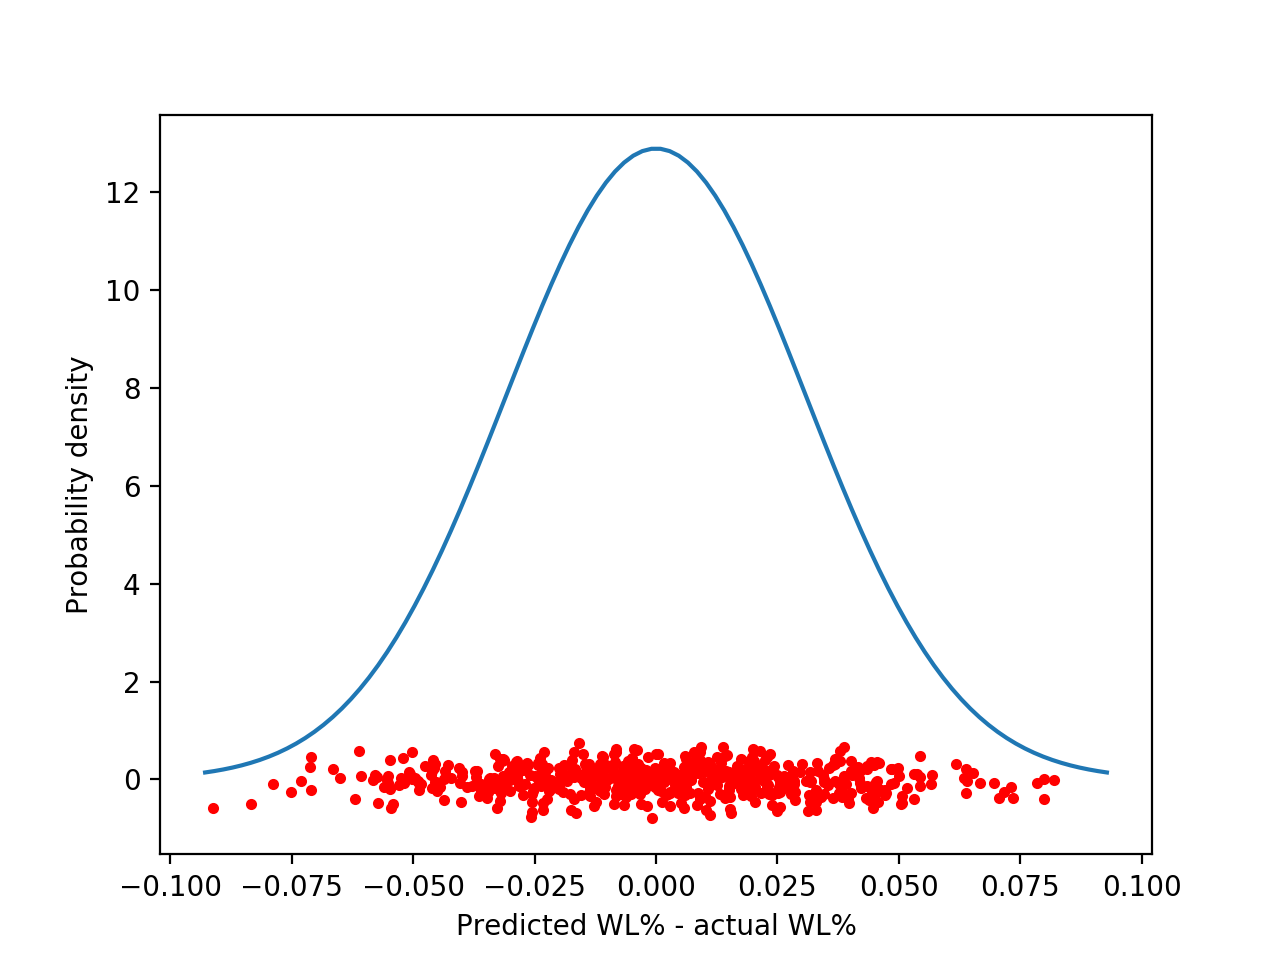
\includegraphics[width=\linewidth]{figure2.png}
  \caption{The Approximate Distribution of Residuals}
  \label{fig:figure2}
\end{figure} 

In sum, we will assume that the distribution of a team's win-loss percentage is normal with mean $\frac{W}{162} + .294$ (where W is team WAR) and variance $.0958\%$, the historical variance of the difference between WAR predicted W-L\% and actual W-L\%. Alternatively, you could use the actual linear regression to find the mean if you believe that WAR is constructed inaccurately. This model is not perfect; for example, it assigns non-zero probabilities to winning negative games. However, it appears to be a decent fit for our purposes.

\subsection{Playoff Odds}

Next, we must figure out how win-loss percentage determines playoff odds. As stated above, we will ignore other teams (treating them as random rather than looking at their projected performance). Teams can make the playoffs in one of two ways: by winning the division or by securing a wild card birth.\\\\
I decided to create 600 fictional teams with win percentages ranging from 0 all the way to 1. Drawing upon historical data, I determined the proportion of divisions each fictional team would have won over the past 20 years. I did the same for the wild card. I then plotted the proportions, treating them as probabilities, and found two curves to approximate the historical probabilities. I fit the curves by inspection, and as displayed in figure 3, the curves model the historical probabilities well. However, this model is not as precise as it looks. The fictional teams are competing with 30 rather than 29 other teams. To compensate for this a little bit, the fictional team wins every tie. While the model is a little off, it should be a decent fit to reality.

\begin{figure}
  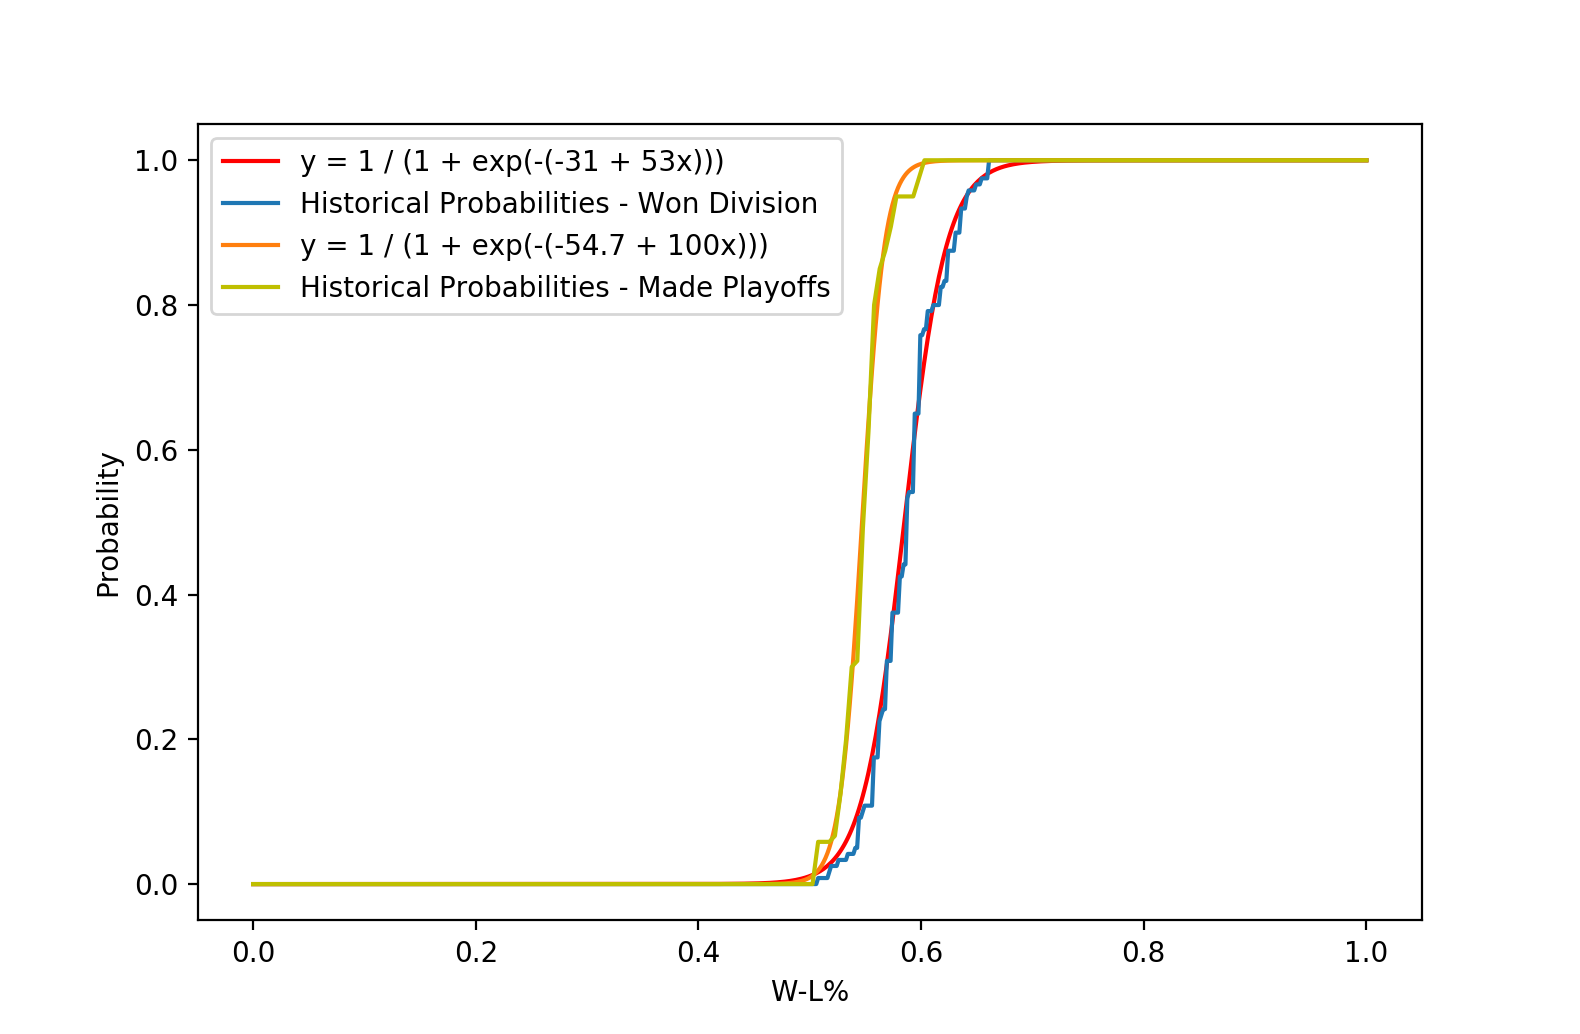
\includegraphics[width=\linewidth]{figure3.png}
  \caption{Playoff Odds From W-L\%}
  \label{fig:figure3}
\end{figure} 

\subsection{World Series Outcome}

Lastly in this section, I fit a logistic curve to the World Series outcomes of teams that made the playoffs, putting team WAR on the x-axis. It would have been more precise to predict playoff opponents, condition on each possible outcome, and go round by round; however, there is simply not enough historical data to make this an easy task. Figure 4 shows the logistic regression curve.

\begin{figure}
  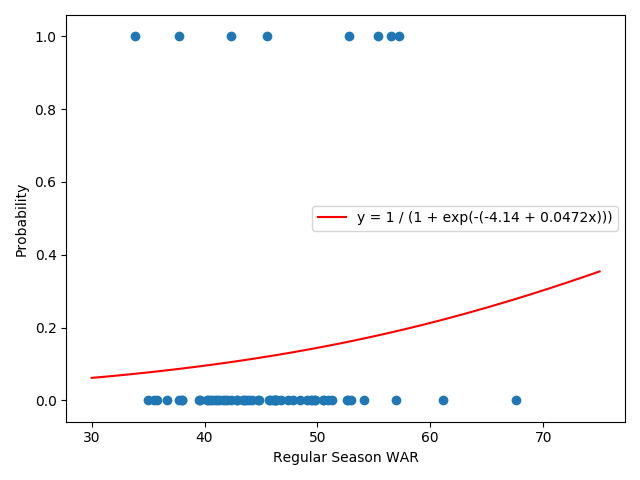
\includegraphics[width=\linewidth]{figure4.png}
  \caption{Logistic Regression of World Series Outcome From WAR}
  \label{fig:figure4}
\end{figure} 

\section{Win Sums}

For the near future, we have many methods to try to predict the sum of a team's WAR. FanGraphs uses a mixture of predictions about a team's depth chart and predictions about the players. We know just about all the players, which simplifies the situation quite a bit. However, simply assigning a predicted WAR total is not exactly what we're after. We want to know what that distribution looks like. This is a practical challenge.\\\\
We will treat $S_i$ as a random variable. As shown before, $S_i$ is the sum of player win contributions. To practically figure out this distribution, we will look at historical data.
%TODO I should probably do some dat analysis here, looking at historical player WAR distributions. They're likely lognormal, with some chance of being zero.

\section{Predicting the Far Future}

We may know what a team's roster will look like next year, but what will it look like in two years? Or ten years? We don't need to know exactly what the roster will be to understand the probability distribution of the sum of each player's win contributions, however.\\\\
All players on an MLB roster are brought onto that roster in 1 of 3 ways. A player can be acquired though (1) free agency, (2) a trade, or (3) promotion from the farm system. The farm system includes in it players acquired in the MLB draft in addition to some other methods like international amateur free agency. The Rule 5 draft complicates these classifications a bit, so we will ignore it; its effect should not be large as the players in the rule 5 draft are not usually far above replacement level.

\end{document}